\documentclass[journal=esthag,manuscript=article]{achemso}
%%%%%%%%%%%%%%%%%%%%%%%%%%%%%%%%%%%%%%%%%%%%%%%%%%%%%%%%%%%%%%%%%%%%%
%% Place any additional packages needed here.  Only include packages
%% which are essential, to avoid problems later. Do NOT use any
%% packages which require e-TeX (for example etoolbox): the e-TeX
%% extensions are not currently available on the ACS conversion
%% servers.
%%%%%%%%%%%%%%%%%%%%%%%%%%%%%%%%%%%%%%%%%%%%%%%%%%%%%%%%%%%%%%%%%%%%%
\usepackage[T1]{fontenc}       % Use modern font encodings
\usepackage[utf8]{inputenc}
\usepackage{todonotes}

%%%%%%%%%%%%%%%%%%%%%%%%%%%%%%%%%%%%%%%%%%%%%%%%%%%%%%%%%%%%%%%%%%%%%
%% If issues arise when submitting your manuscript, you may want to
%% un-comment the next line.  This provides information on the
%% version of every file you have used.
%%%%%%%%%%%%%%%%%%%%%%%%%%%%%%%%%%%%%%%%%%%%%%%%%%%%%%%%%%%%%%%%%%%%%
%%\listfiles

%%%%%%%%%%%%%%%%%%%%%%%%%%%%%%%%%%%%%%%%%%%%%%%%%%%%%%%%%%%%%%%%%%%%%
%% Place any additional macros here.  Please use \newcommand* where
%% possible, and avoid layout-changing macros (which are not used
%% when typesetting).
%%%%%%%%%%%%%%%%%%%%%%%%%%%%%%%%%%%%%%%%%%%%%%%%%%%%%%%%%%%%%%%%%%%%%
\newcommand*\mycommand[1]{\texttt{\emph{#1}}}


%%%%%%%%%%%%%%%%%%%%%%%%%%%%%%%%%%%%%%%%%%%%%%%%%%%%%%%%%%%%%%%%%%%%%
\author{Eduard Szöcs}
\affiliation[Institute for Environmental Sciences]{Institute for Environmental Sciences, University of Koblenz-Landau, Germany}
\email{szoecs@uni-landau.de}
\phone{+49 (0)6341 280 31552}

\author{Marvin Brinke}
\affiliation[German Federal Institute of Hydrology]{German Federal Institute of Hydrology (BfG), Koblenz, Germany}

\author{Bilgin Karaoglan}
\affiliation[German Federal Environmental Agency]{Federal Environmental Agency (UBA), Dessau-Roßlau, Germany}

\author{Ralf B. Schäfer}
\affiliation[University Koblenz-Landau]{Institute for Environmental Sciences, University of Koblenz-Landau, Germany}


%%%%%%%%%%%%%%%%%%%%%%%%%%%%%%%%%%%%%%%%%%%%%%%%%%%%%%%%%%%%%%%%%%%%%
\title[Pesticides small streams]{Pesticides pollution of small streams in Germany}
\abbreviations{mo, pest, ger, tu}
\keywords{Monitoring, Pesticides, Germany, Toxic Units, Freshwater}


%%%%%%%%%%%%%%%%%%%%%%%%%%%%%%%%%%%%%%%%%%%%%%%%%%%%%%%%%%%%%%%%%%%%%
\begin{document}
%%%%%%%%%%%%%%%%%%%%%%%%%%%%%%%%%%%%%%%%%%%%%%%%%%%%%%%%%%%%%%%%%%%%%
%% The "tocentry" environment can be used to create an entry for the
%% graphical table of contents. It is given here as some journals
%% require that it is printed as part of the abstract page. It will
%% be automatically moved as appropriate.
%%%%%%%%%%%%%%%%%%%%%%%%%%%%%%%%%%%%%%%%%%%%%%%%%%%%%%%%%%%%%%%%%%%%%
\begin{tocentry}

Some journals require a graphical entry for the Table of Contents.
This should be laid out ``print ready'' so that the sizing of the
text is correct.

Inside the \texttt{tocentry} environment, the font used is Helvetica
8\,pt, as required by \emph{Journal of the American Chemical
Society}.

The surrounding frame is 9\,cm by 3.5\,cm, which is the maximum
permitted for  \emph{Journal of the American Chemical Society}
graphical table of content entries. The box will not resize if the
content is too big: instead it will overflow the edge of the box.

This box and the associated title will always be printed on a
separate page at the end of the document.

\end{tocentry}



%%%%%%%%%%%%%%%%%%%%%%%%%%%%%%%%%%%%%%%%%%%%%%%%%%%%%%%%%%%%%%%%%%%%%
\begin{abstract}
Fehlt noch...
\end{abstract}


%%%%%%%%%%%%%%%%%%%%%%%%%%%%%%%%%%%%%%%%%%%%%%%%%%%%%%%%%%%%%%%%%%%%%
\section{Introduction}

More than 50\% of the total land area in Germany are used by agriculture \citep{statistisches_bundesamt_bodenflache_2014}.
In the year 2014 more the 45000 tonnes of 766 authorized pesticides were sold for application on these areas \citep{bundesamt_fur_verbraucherschutz_und_lebensmittelsicherheit_absatz_2015}.
The applied pesticides may enter surface waters via spray-drift, edge-off-field run-off or drainage, with run-off being one of the major input routes \citep{schulz_comparison_2001}.
Once entered the surface waters pesticides are frequently detected in environmental monitoring \citep{malaj_organic_2014} and may have adverse effects on biota and ecosystem functioning \citep{schulz_field_2004, schafer_effects_2007}.



% Small waterbodies

% runoff during rainfall (Liess et al. 1999)

% underestiamtion of grab sampling (Stehle et al. 2013). 


The aim of this study was 
(i) to compile monitoring data on a national scale and to answer the questions: \\
(ii) Is the data a representative description of the pollution situation? \\
(iii) Are small agricultural waters more polluted compared to bigger streams? Are there thresholds? \\
(iv)  How polluted are small streams and which pesticides are responsible?


\section{Methods}
\subsection{Data compilation}

We queried chemical monitoring data of pesticides from sampling sites with catchment size $\mathrm{< 100km^2}$ for the years 2005 to 2015 from all 13 non-city federal states of Germany.
Additionally, we compiled data available from previous studies and searched online databases.
This yielded to a total of more then 30 datasets of different formats.

We homogenized and unified these datasets into a common database.
We implemented a robust and transparent data cleaning work flow \citep{poisot_best_2015}, though parts of the dataset are proprietary.
An overview of the data cleaning process is provided in the supplemental materials.  
The compiled dataset comprised only a small fraction of standing waters and most of the samples where sampled via grab sampling.
Therefore, we report  only results for grab sampling from streams.  \todo{move to results and say that nearly no information on standing waters is available}
To assess whether  grab samples were taken during potential rainfall events we intersected sampling coordinates with daily precipitation data \citep{rauthe_central_2013} from the sampling date and the day before .

\subsection{Characterization of chemical pollution}
We characterized chemical pollution using three indicators:

\begin{enumerate}
\item National and international Environmental Quality Standards (EQS) \citep{ogewv_verordnung_2011,european_union_directive_2013}:
We used only Maximum Annual Concentration EQS (MAC-EQS) for characterization.

\item Regulatory Acceptable Concentrations (RAC) \citep{brock_linking_2010}:
This is the lowest concentration at which no acceptable biological effects are expected. 
These are derived during authorization  process of pesticides and contain an uncertainty factor.
The German Federal Environmental Agency provided RACs for this study.  
We expressed  RAC as Risk Quotient (RQ)

\begin{equation}
RQ = \frac{C}{RAC}
\end{equation}

Where $C$ is the concentration of a compound in a sample.

\item Maximum Toxic Units ($\mathrm{TU_{max}}$)  \citep{sprague_measurement_1970}: 
\begin{equation}
TU_{max} = max(\frac{C_i}{EC_{50, D.magna, i}})
\end{equation}

Where $C_i$ is the concentration of compound $i$ in a sample and $EC_{50, D.magna, i}$ is the concentration of this compound where 50\% of the exposed animals showed after 48 hours an effect in a laboratory study.
We compiled $EC_{50, D.magna}$ values from literature \citep{malaj_organic_2014}, databases \citep{pesticide_action_network_pan_2015,u.s._epa_ecotoxicology_2015} or model predictions \citep{schuurmann_quantitative_2011}, where experimental data had priority.
We used the maximum TU per sample, as it is independent of the number of measured compounds and makes no assumptions on the mode of action.
A table of all included compounds can be found in the supplement.
\end{enumerate}


\subsection{Characterization of catchments}
We delineated catchments upstream of the sampling sites using a digital elevation model \citep{eea_digital_2013} and a multiple flow direction algorithm \citep{holmgren_multiple_1994} as implemented in GRASS GIS 7 \citep{neteler_grass_2012}.
Catchment delineation has been manually checked for accuracy. 
In areas with low relief energy the delineation algorithm did not produce accurate results and we used river catchments provide by federal state authorities in these cases.
For each catchment we calculated the relative coverage (\%) with agricultural areas based on Official Topographical Cartographic Information System (ATKIS) of the land survey authorities.


\subsection{Statistical analyses}

We used Multidimensional Scaling (MDS) based on jaccard dissimilarity in conjunction with hierarchical clustering to display differences in the spectra of analysed compounds per federal state.




\section{Results}
\subsection{Overview and representativeness of compiled data}

We compiled a national scale dataset  comprising 42236 samples from 3049 sampling sites (Figure \ref{fig:fig1} and Supplement). 
We found big differences in the number of sampling sites between federal states.

The dataset include 484 



\begin{figure}
  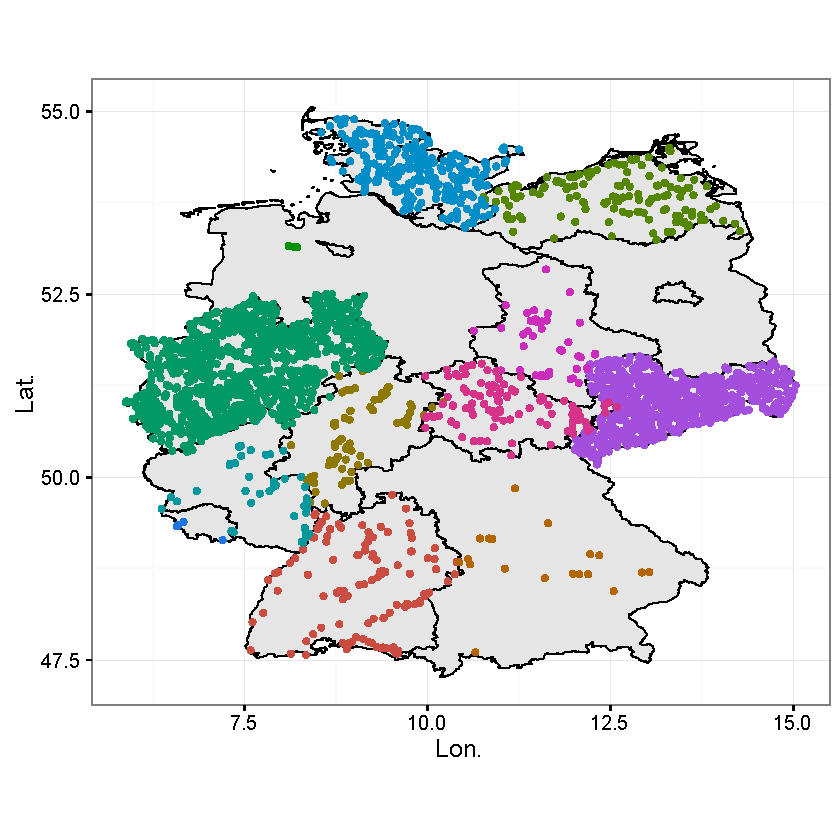
\includegraphics[width=.8\textwidth]{fig/fig1.pdf}
  \caption{Spatial distribution of the 3109 sampling sites. Colour codes different federal states.}
  \label{fig:fig1}
\end{figure}

\begin{figure}
  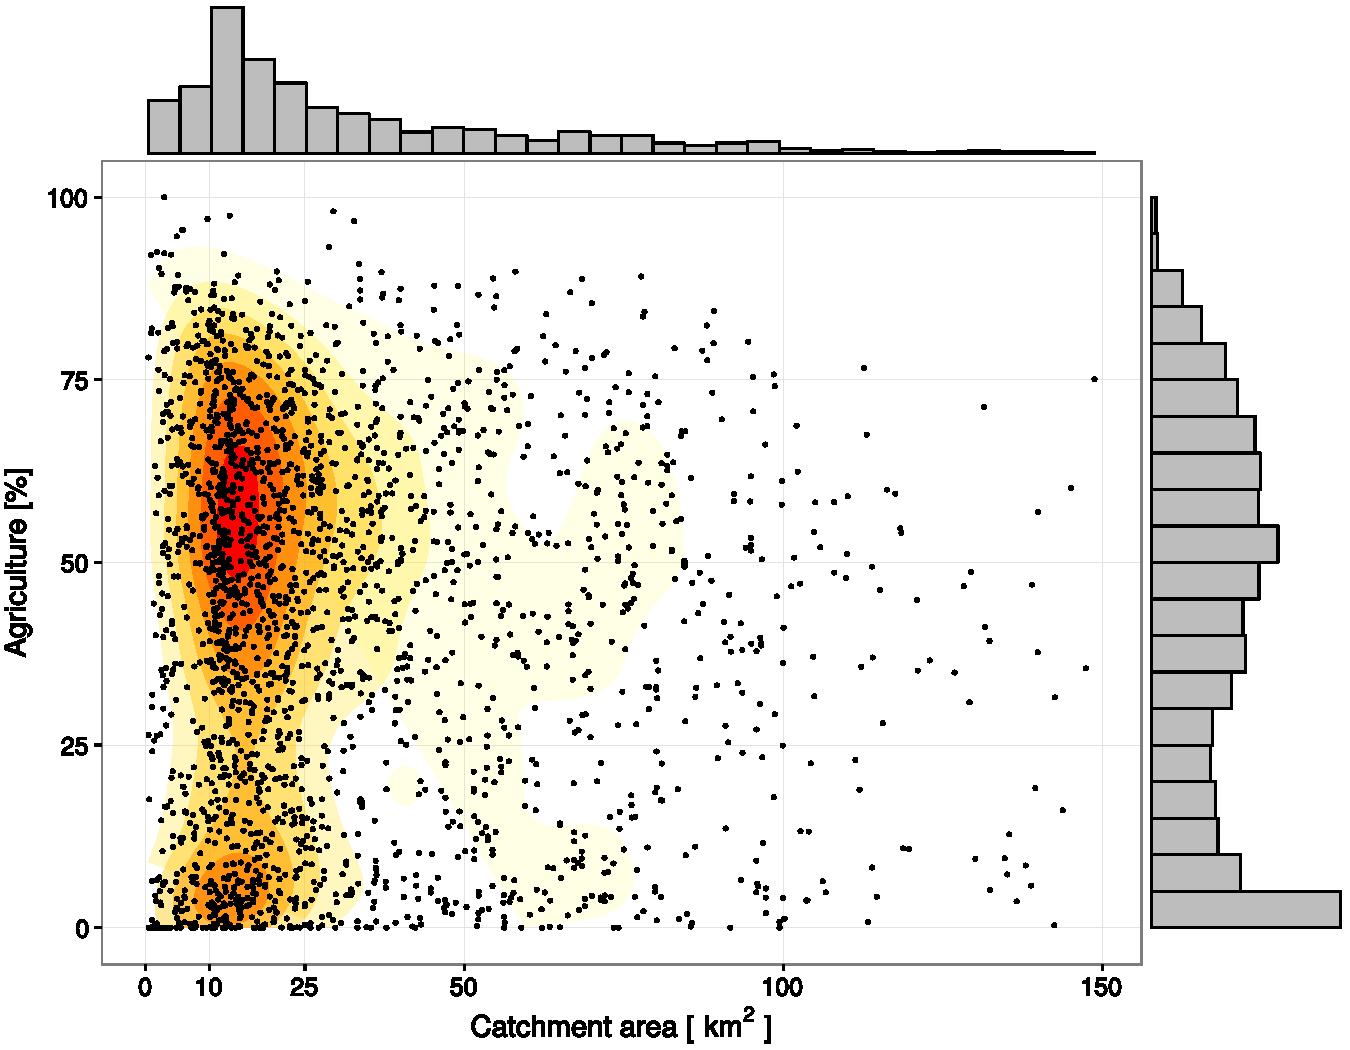
\includegraphics[width=.8\textwidth]{fig/ezg_lu.pdf}
  \caption{Distribution of catchment area and agriculture within the catchment area across the sampling sites.
  Only sampling sites with catchment area < 150 km\textsuperscript{2} are displayed. 
  Colour codes the 2-dimensional density of points.
  }
  \label{fig:fig_ezg_lu}
\end{figure}


\subsection{Are small agricultural waters more polluted compared to bigger streams?}




\subsection{Pesticide pollution of small streams}




\section{Discussion}

Vergleich mit der Schweiz.....

\subsection{Subsection}






%%%%%%%%%%%%%%%%%%%%%%%%%%%%%%%%%%%%%%%%%%%%%%%%%%%%%%%%%%%%%%%%%%%%%
\begin{acknowledgement}
The authors thank the authorities for providing chemical monitoring data and the German Federal Environmental Protection Agency (UBA) for funding this project.
\end{acknowledgement}


%%%%%%%%%%%%%%%%%%%%%%%%%%%%%%%%%%%%%%%%%%%%%%%%%%%%%%%%%%%%%%%%%%%%%
\begin{suppinfo}
The following files are available free of charge.
\begin{itemize}
  \item Supplemental\_Materials.pdf : Supplemental Materials
\end{itemize}
\end{suppinfo}



%%%%%%%%%%%%%%%%%%%%%%%%%%%%%%%%%%%%%%%%%%%%%%%%%%%%%%%%%%%%%%%%%%%%%
\bibliography{references}

\end{document}
